\chapter{Einführung in Internet of Things}
\section{Übersicht}
Das Internet der Dinge unterscheidet sich in einigen Aspekten vom klassischen Internet. End-Benutzer haben über sogenannte Terminals wie Laptops oder Smartphones über die globale Internet Infrastruktur kommuniziert \cite{MiorandiSicariPellegriniChlamtac12}. Diese Terminals wurden meist von Benutzern eingeschaltet, benutzt und wieder ausgeschaltet. Damit Geräte mit dem Internet auf sinnvolle Art und Weise kommunizieren konnten, war eine manuelle Tätigkeit von Benutzern notwendig \cite{Radovici15}. Beispiele dafür sind das Abrufen von E-Mails, Surfen im Web, Streaming von Videos oder Spielen von Online Games \cite{MiorandiSicariPellegriniChlamtac12}.

Mit \glqq Internet of Things\grqq{} (IoT) wird eine andere Philosophie verfolgt. Es gibt keine einheitliche Definition und Abgrenzung von IoT. Grundsätzlich versucht man Objekte und Gegenstände, welche im klassischen Sinne des Internets nicht berücksichtigt wurden, ans Netz anzuschliessen. Mit minimalen menschlichen Eingriffen sollen diese Geräte Daten sammeln, austauschen und aufgrund von Software und Algorithmen Entscheidungen treffen \cite{RoseEldridgeChapin15}. Man spricht im Zusammenhang von \glqq Things \grqq{} auch von \glqq Smart Devices\grqq{} oder \glqq Smart Objects\grqq .
\subsection{Smart Objects}
Smart Objects oder auch \glqq Things\grqq{} ergänzen das herkömmliche Internet um eine Vielzahl neuartiger Teilnehmer. Man ist versucht, die mit dem Internet erschaffene virtuelle Welt mit Objekten der tatsächlichen \glqq echten\grqq{} Welt zu verbinden. Der Begriff \glqq Smart\grqq{} ist seit der Erscheinung des iPhones weltweit bekannt. Er beschreibt die Fähigkeit eines Objekts mit dem Internet zu kommunizieren. 

Während Smartphones oder Smart-TVs noch als herkömmliche Internet Terminals angesehen werden können, so erweitern die Smart Objects das bisherige Internet um eine neue Art von Teilnehmer. Smart Objects lassen sich wie folgt beschreiben:
\begin{itemize}
\item	haben eine physikalische Repräsentation mit Eigenschaften wie Form und Grösse
\item	haben Mindestmass an Kommunikationsfunktionalitäten wie Request/Reply
\item	besitzen eine UID (unique identifier)
\item	haben mindestens einen Namen und eine Adresse
\item	besitzen ein Mindestmass an Rechenfähigkeiten
\item	besitzen Sensoren, um physikalische Erscheinungen wie Druck, Licht, Temperatur, etc. zu messen
\end{itemize}

Der letzte Punkt in der oberen Definition beschreibt den tatsächlichen Unterschied zu herkömmlichen Devices im Internet. Konzeptionell liegt bei IoT der Fokus mehr auf Daten und Informationen von physikalischen Objekten als bei Punkt-zu-Punkt Kommunikation von Terminals \cite{MiorandiSicariPellegriniChlamtac12}.

\section{Einsatzgebiete}
''Internet of Things'' hat extrem viele Einsatzmöglichkeiten und wir stehen erst am Anfang. Es werden immer neue Einsatzbereich entdeckt und vorhandene erweitert und optimiert. Um die Einsatzmöglichkeiten aufzuzeigen, wird hier das Beispiel ''Gesundheitsvorsorge'' genauer gezeigt.
\subsection{Zuhause}
\subsection{Beim Doktor}
\subsection{Im Spital}
\subsection{•}
\section{Sensortypen}
Beim Thema ''Internet of Things'' spielen die Sensoren eine zentrale Rolle. Es gibt viele verschiedene Typen von Sensoren, welche unterschiedlichste Daten liefern und man muss daher wissen, wie man mit dem jeweiligen Sensortyp umgeht. 
\subsection{Temperature}
Temperatursensoren werden in vielen Gebieten eingesetzt. Häufig wird dieser Sensortyp zur Überwachung von Gebäuden eingesetzt, oder hilft bei maschinell hergestellten Esswaren, die richtige Temperatur zu halten. Auch kann ein Bauer diese Sensoren verwenden, um die Bodentemperatur zu Überwachen. So kann man effizienter und gewinnbringender Arbeiten, ohne selber Messungen durchzuführen. 
\subsection{Acceleration/Tilt}
Beschleunigungs- und Lagesensoren hat wohl jeder in seiner Hosentasche. Nahezu alle neuen Smartphones haben solche eingebaut. Auch in der Autoindustrie findet man solche sehr häufig. Durch solche Sensoren kann man viele Verschiedene Daten erhalten. So kann man zum Beispiel Bewegungsprofile einer Person erstellen und den Fitnesslevel bestimmen.
\subsection{Acoustic/Sound/Vibration}
Nicht nur in der Musikbranche sind Akustik- und Soundsensoren sehr wichtig. So wird auch der Lärm in einem Gebiet oder in einer Stadt gemessen, um Verbesserungen der Lebensqualität zu erreichen. Sehr wichtig sind auch die Vibrationssensoren, welche wichtige Daten zu Unterwassererdbeben senden. So können Tsunamis immer früher erkannt werden und retten Leben. 
\subsection{Chemical/Gas}
Chemikaliensensoren werden häufig in den Städten mit viel Verkehrsaufkommen eingesetzt. Dadurch wird die Luftqualität bestimmt. Auch in Laboren ist dies ein wichtiger Sensor, um die Qualität oder Reinheit von Gasen zu messen.
\subsection{Electric/Magnetic}

\subsection{Flow}
Für die Überwachung von Flüssen oder Wasserleitungen werden Flusssensoren verwendet. So können zum Beispiel Wasserversorger den Verbrauch jedes Haushalts über das Internet messen lassen und müssen nicht vor Ort die Zähler ablesen. Oder auch für die Überwachung von Flüssen kann dieser Sensor verwendet werden. So wird man bei zu schnellen und zu vielem Wasser vor Überschwemmungen gewarnt.
\subsection{Force/Load/Torque/Strain/Pressure}

\subsection{Humidity/Moisture}
Ein wichtiger Bestandteil der Luftqualität ist auch die Luftfeuchtigkeit. Diese wird mit diesem Typ gemessen. So können Smart Buildings die Luftfeuchtigkeit laufend messen und immer wieder optimieren. Auch in der Landwirtschaft kann so eine Automation eingeführt werden, damit die Erde immer optimal bewässert ist.
\subsection{Leaks/Levels}
Lecks- und Levelsensoren sind zum Beispiel in der Landwirtschaft notwendig. Die Landwirtschaft benötigt  viel Wasser und man möchte unnötige Lecks vermeiden. Ein weiterer wichtiger Einsatzbereich ist die Überwachung von Flüssigkeitsständen, zum Beispiel bei Staudämmen oder in Lagersystemen.
\subsection{Machine Vision / Optical Ambient Light}

\subsection{Motion/Velocity/Displacement}

\subsection{Position/Presence/Proximity}
Immer wichtiger wird auch dieser Typ von Sensoren. Durch die Bestimmung von Distanzen oder der Position in einem Raum, ergeben sich viele Einsatzmöglichkeiten. Ein bekanntes Beispiel ist der Abstandssensor bei Autos, um Parkschäden oder Auffahrunfälle zu vermeiden. Oder auch die Gebäudeüberwachung profitiert durch solche Sensoren, da man mehrere Gebäude zentral Überwachen kann.
\section{Kommunikation}
Internet of Things verbindet Objekte aus der realen Welt miteinander. Um Objekte aus der Realität in die virtuelle Welt zu transformieren, werden Sensoren verwendet. Es gilt nun, diese Sensoren mit dem Internet zu verbinden.

Um unterschiedliche Bedürfnisse abzudecken, sind verschiedene Arten der Kommunikation entstanden. Die mit Sensoren ausgestatteten Geräte können sich in ihrer Weise, mit dem Internet zu kommunizieren stark unterscheiden.

\subsection{Modelle}

\subsection{Architektur}
Man könnte ein IoT System in vier wichtige Gruppen unterteilen: [micrium]
\begin{itemize}
\item Dinge (things)
\item das lokale Netzwerk
\item das Internet
\item Back-End Services (z.B. Cloud Services)
\end{itemize}
\\
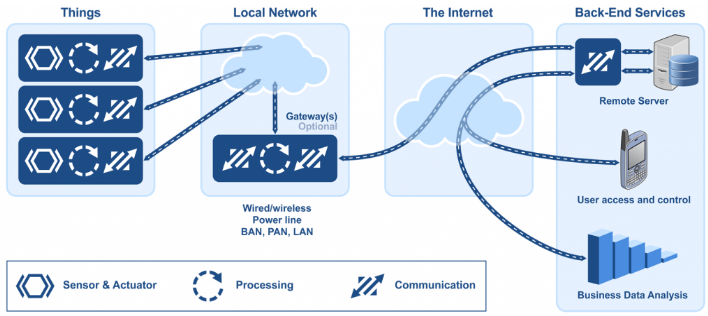
\includegraphics[scale=0.8]{images/iot_system_overview_by_micrium.PNG}
\\
Grundsätzlich scheint die Architektur vertraut. Smart Objects kommunizieren über ein lokales Netzwerk mit Diensten im Internet.

Bisher konnten Geräte wie Laptops, PCs und Smartphones beinahe einheitlich mit dem Internet verbunden werden; entweder verkabelt über Ethernet oder drahtlos über ein lokales WLAN oder mobile Netze wie UMTS und LTE. Die Endgeräte verfügten jeweils über viel Rechenleistung, Speicher und ein leistungsfähiges Betriebssystem mit einem vollständig implementierten TCP/IP Stack. 

In einem IoT System muss man von einer grossen Anzahl an Geräten mit Sensoren ausgehen. Diese Geräte verfügen meist über eine extrem niedrige Bandbreite, wenig Speicher und Rechenleistung [youtube].
\subsection{Wireless Sensor Netzwerke}
Bei einer Vielzahl von verbundenen Sensoren, welche über einen grossen Bereich verstreut sind, bietet sich ein Wireless Sensor Network (WSN) an. In einem WSN werden die Sensoren nicht direkt mit dem Internet verbunden. Die Daten werden drahtlos von Teilnehmer zu Teilnehmer versendet. Muss ein Datenpaket in ein entferntes Netzwerk wie das Internet, so wird ein Gateway oder Edge Node benötigt.
\\
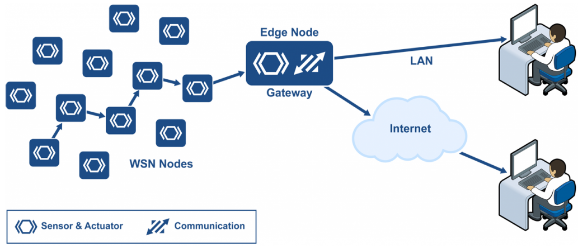
\includegraphics[scale=0.8]{images/iot_wsn_lan_overview_by_micrium.PNG}
\\
WSN Nodes sind typischerweise günstig im Einkauf. Sie können mit sehr wenig Leistung betrieben werden, dies ermöglicht den Batteriebetrieb. Durch diese Eigenschaften können WSN Nodes einfach, schnell und in sehr grosser Anzahl bereitgestellt werden. 
\section{Security Aspekte}

